\documentclass[border=4pt]{standalone}
\usepackage{amsmath}
\usepackage{tikz}
\usetikzlibrary{arrows}
\begin{document}
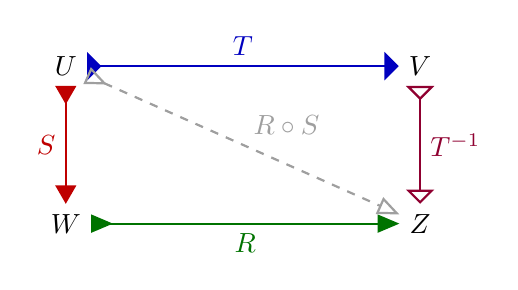
\begin{tikzpicture}[x=15mm,y=10mm,line width=.8pt]
  \node (u) at (0,2) {$U$};
  \node (v) at (3,2) {$V$};
  \node (w) at (0,0) {$W$};
  \node (z) at (3,0) {$Z$};

  \draw[blue!75!black,{triangle 90 reversed}-{triangle 90}]
    (u) -- node[above] {$T$} (v);
  \draw[red!75!black,{triangle 60 reversed}-{triangle 60}]
    (u) -- node[left] {$S$} (w);
  \draw[green!45!black,{triangle 45 reversed}-{triangle 45}]
    (w) -- node[below] {$R$} (z);
  \draw[purple!75!black,{open triangle 90 reversed}-{open triangle 90}]
    (v) -- node[right] {$T^{-1}$} (z);
  \draw[gray!75,{open triangle 45 reversed}-{open triangle 45},dashed]
    (u) -- node[above right] {$R\circ S$} (z);
\end{tikzpicture}
\end{document}
